\chapter{Introduction}
This project is about machine learning of different statistical classifiers.
Machine learning is about construct and study systems that can learn from data.
This could be used to train a system to recognize patterns in, for instance, emails and learn how to distinguish between spam and non-spam messages. In this project the classifiers are applied to reviews and the task is to categorize these.
By statistical analysis of experiments, the classifiers are compared in terms of, for instance, classification accuracy.
\section{Problem description}
The problem is to categorize reviews from Amazon. There are 6 different categories;
books, camera, DVD, health, music and software. The reviews are also
categorized as positive and negative reviews. 



The following classification tasks should be investigated using different classification:
\begin{itemize}
\item Text categorization: Categorize review documents into their six categories: Books, DVDs, Cameras, Music, Health, and Software.
\item In-domain sentiment analysis: For each review category, train and classify review documents as positive or negative. 
\item  Out-of-domain sentiment analysis: Make training and test sets for two different topics (such as Books and Cameras).
\end{itemize}
The question of issue in this project is to answer weather there is a correlation between Out-of-domain sentiment analysis and Text categorization. 


%The classification is done by
%implementing five different classification algorithms; Naive Bayes, Perceptron,
%Averaged Perceptron, K-nearest neighbours (KNN) and Support vector machine
%%(SVM).
%\\\\ There is three different kinds of classification tests that should
%be done:
%\begin{itemize}
%\item In-domain sentiment analysis - For each category, train and classify documents as positive or negative
%\item Out-of-domain sentiment analysis - Train on one category and test on another
%\item Text categorization - categorize the documents into their categories
%\end{itemize}
Before classifying the input data, which is given as text files, the data must be
converted to a suitable form. Even further there may be irrelevant data
in the text files. Some common words may be totally useless for the classification,
such as ''the'' and ''I''. How should the data be processed to handle this
problem? Some words may also say the same about which category a text belongs to, for instance
words as ''person'' and ''persons''. There are also a lot of data and  a lot of
unique words. Is every unique word really important for the classification
results? Is it possible to remove such words?

%The
%input should be divided in words somehow, either one word (unigrams) or two
%words (bigrams). Some common words are totally useless for the classification,
%such as ''the'' and ''I''. These are called stop-words and should not be a part
%of the input to the algorithms. To get less words it's also possible to use a
%stemmer, such as Snowball to prevent separation of different inflectional
%forms, such as ''person'' and ''persons''. Another way of getting less input
%data is to use Term Frequency–Inverse Document Frequency TF-IDF. TF-IDF is a
%numerical statistic of how important a is in a document.

%Before classifying the input data, which is text files, must be processed. The
%input should be divided in words somehow, either one word (unigrams) or two
%words (bigrams). Some common words are totally useless for the classification,
%such as ''the'' and ''I''. These are called stop-words and should not be a part
%of the input to the algorithms. To get less words it's also possible to use a
%stemmer, such as Snowball to prevent separation of different inflectional
%forms, such as ''person'' and ''persons''. Another way of getting less input
%data is to use Term Frequency–Inverse Document Frequency TF-IDF. TF-IDF is a
%numerical statistic of how important a is in a document.

\section{Theory}
(TEXT HÄR????)
\subsection{Text classification}
Text classification has become a popular subject within machine learning as the amount of information lately has rapidly grown \citep{joachims}. Text classification is to
classify documents into a fixed number of predefined categories. The categories
could be sentimental (positive / negative) or different topics that the
document concern \cite{ngrams_ai}.

\subsubsection{Representing text}
A document is typically a huge string containing all characters and is not
suitable for classification, hence some processing needs to be done on each
document \cite{ngrams_ai}.
\\\\
All words in a document isn't interesting when doing text classification. E.g.
words like "the", "one", "are", "is" are words that will occur in any human
readable text, but has no value when trying to find similarities and
differences between documents. These words are called "stop-words" and are
usually filtered out and treated as noise \cite{joachims}.
\\\\
When working with document, different inflections of a word should be treated
as the same word. There is no need to separate the words "persons" and
"person", because both words give the same information. This is called Stemming
and we will not focus more on the theory behind it \cite{stemming}.
\\\\
There are various ways of storing document and the representation has a big
impact on the result of different classifiers. The Bag-of-words model is a
simplifying model where a text is represented as a unordered set of words,
without respect to grammar or order of words \citep{bag_of_words}.
\\\\
To be able to clasify documents they must
in same way get a numerical presentation. This can be done by builing a
feature vector which is an n-dimensional vector of numerical features
that represents the words.
\subsubsection{Features}
\begin{itemize}
\item Feature size - Sometimes the feature vector can be very large adn hard to
        handle. Then it could be a good idea to just choose the 1000 most
        frequent words or maybe the 100 most frequent words \citep{joachims}.
\item N-grams - N-grams is a sequence of symbols of length $n$, in this case
        words. Unigram is then one word and bigram is two words \citep{ngrams_ai}.
\item TF-IDF - Term Frequency–Inverse Document Frequency, is used to count the
        words in the documents and give a number of how important each word is.
        This is given by Equation~\ref{eq:tfidf} \citep{tfidf}.
\end{itemize}

\begin{equation}
\begin{array}{l}
tf(t,d) = \frac{f(t,d)}{(max \{f(w,d) : w \in d\})} \\
idf(t,D) = log(\frac{|D|}{|\{d \in D : t \in d\}|})
\end{array}
\label{eq:tfidf}
\end{equation}

\subsection{Naive Bayes}
The Naive Bayes classifier uses (naive) independence assumptions to simplify the conditional probability $P(c\vert\mathbf{x})$ of a feature vector $\mathbf{x} \in \mathbb{R}^D$ belonging to class $c$. This is done by using Bayes' rule to formulate $P(c\vert \mathbf{x}) = \frac{P(\mathbf{x}\vert c) P(c)}{P(\mathbf{x})}$ and rewriting as follows.
\begin{align*}
P(c\vert \mathbf{x}) &\propto P(\mathbf{x}\vert c)P(c)
\\&=P(c,\mathbf{x})
\\&\propto P(c) P(x_1,...,x_D\vert c)
\\&\propto P(c) P(x_1\vert c) P(x_2,...,x_D\vert c, x_1)
\\&\propto P(c) P(x_1\vert c) P(x_2\vert c, x_1) P(x_3,...,x_D\vert c,x_1,x_2)
\\&\propto P(c) P(x_1\vert c) P(x_2\vert c, x_1) P(x_3\vert c,x_1,x_2) \dots P(x_D\vert c, x_1,...,x_{D-1})
\\&\dots
\end{align*}
The independence assumption says that each feature $x_i$ is independent of every other feature $x_j,..,x_k$, rendering $P(x_i\vert x_j,...,x_k) = P(x_i\vert c)$, which translates the posterior $P(c\vert \mathbf{x})$ to
\begin{align}
P(c\vert \mathbf{x}) &\propto P(c) P(x_1\vert c) P(x_2\vert c) \dots P(x_D\vert c) \nonumber
\\&= P(c) \prod_{i=1}^{D} P(x_i\vert c).\label{eq:naivebayes_model}
\end{align}
A suitable choice for each conditional distribution $P(x_i\vert c)$ is the \textit{maximum likelihood estimate}, MLE, which corresponds to the relative frequency of each parameter in the training data.
\\\\
The classification procedure then calculates the \textit{maximum a posteriori} (MAP) class $c_{\textit{map}} = \argmax_{c\in C} P(c\vert \mathbf{x})$. Since the argument $c$ that maximizes $P(c\vert \mathbf{x})$ also maximizes $\log P(c\vert \mathbf{x})$, the product in Equation \ref{eq:naivebayes_model} can be written as a sum of log terms, which helps to avoid arithmetic underflow. The pseudocode for the classification procedure is shown in Algorithm \ref{algorithm:naive_bayes_classification}.

\begin{algorithm}[h]
 \SetAlgoLined
 \SetKwInOut{Input}{input}\SetKwInOut{Output}{output}
 \KwData{\textit{Feature vector with unknown class} $\mathbf{x} \in \mathbb{R}^D$; \textit{Class weights} $\{P(c) : c \in C\}$; \textit{Conditional feature probabilities} $\{P(x_1\vert c), ..., P(x_D\vert c)\}$}
 \KwResult{Classification for $\mathbf{x}$}
 \ForEach{$c \in C$}
 {
score[$c$] $\leftarrow \log P(c)$\\
\For{$i=1$ \KwTo $D$}
{
	score[$c$] += $\log P(x_i\vert c)$
}
 }
 \Return $\displaystyle \argmax_{c \in C} score[c]$ \\

 \caption{Multinomial Naive Bayes classification algorithm}
 \label{algorithm:naive_bayes_classification}
\end{algorithm}

\subsection{K-Nearest Neighbour (KNN) algorithm}
%http://www.cse.chalmers.se/edu/course/TDA231/mlsli11.pdf
K-nearest neighbours (KNN) algorithm is one of the simplest machine learning
algorithms. The classification performed by KNN works as follows: Fix some
number $k$. For any new $x \in X$, take the most common classification value among
the $k$ training examples in $D$ closest to $x$ \cite{ml_2011}.
\\\\
Even though the KNN algorithm
seems extraordinary simple there are some things that one must take in
consideration. First of all what is nearest? There is of course a natural
distance function in a geometrical space but a proper definition in parameter
space is not obvious. As it turn out a distance function can be defined in a lot
of ways. The given attributes are overall very different in reality.
One may multiply each attribute variable by arbitrary factors or in other
words stretch the coordinate axes arbitrary and independent. It is very easy to
find examples when doing so will result in very different outcomes of the classifications.
Even further irrelevant attributes may change the classification even though they
shouldn't do so. This phenomena is called \emph{curse of dimensionality}. One
can try to find good stretch factors by performing cross validation \cite{ml_2011}.
\\\\
%An other problem is the computation complexity. KNN is sad to have a lazy
%learning method. In other words it does output hypotheses in explicit form.
%Instead a lot of computational steps are required for the classification.
%\\\\
A further issue is to find a suitable $k$. A great choose of $k$ various
depending on many circumstances. A keystone is that if the training set is large
it is important to get rid of noise in the data, hence increase $k$. On the other
hand a big $k$ requires more calculation. There are however also other more
complex ways for reducing noise \cite{ml_2011}.
%https://dl.dropbox.com/u/5139428/ml-course/Classification1.pdf

\begin{figure}[h!]
\centering
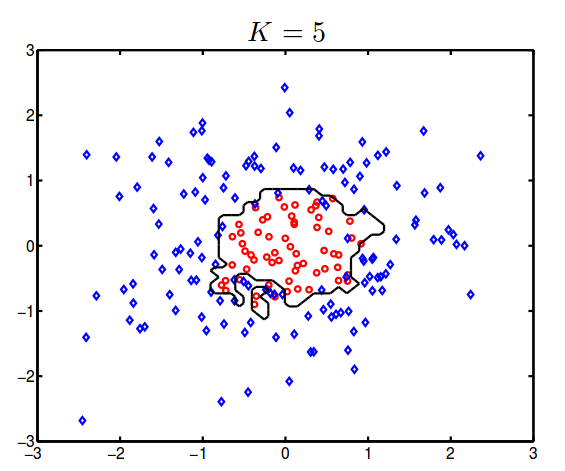
\includegraphics[scale=0.3]{../Plottar/KNN.png}
\caption{A classification done by KNN, $k = 5$.}
\label{fig:knn}
\end{figure}

\subsection{Support Vector Machine (SVM)}
Support Vector Machines (SVM) constructs a non-probabilistic linear classification separating exactly two different classes of input data. Given some input data SVM outputs a hyperplane which separates the given data depending on its class. SVM chooses the hyperplane which has the largest distance between the two classes. This distance is refered to as the margin in Figure~\ref{fig:svm}. In general the larger margin, the lower generalization error. \citep{svm_ai} \\\\
The data points that is at the margin distance from the hyperplane is called the support vectors, shown in Figure~\ref{fig:svm}.. The constructed hyperplane only depends on the support vector, meaning that SVM is dimensional independent.
\begin{figure}[h!]
\centering
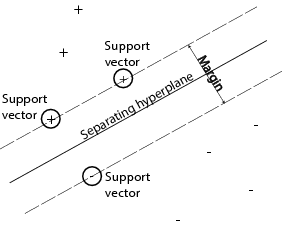
\includegraphics[scale = 0.7]{../Plottar/svmhyperplane.png}
\caption{Example of SVM. Support vectors are marked with dots \citep{svm_picture}. }
\label{fig:svm}
\end{figure} \\
The equation of the hyperplane is given by
\begin{equation}
w \cdot x + b = 0
\end{equation}
where the training data points are $x_i \in R^d$ with labels $y_i \pm 1$. $s_i$ is a slack variable and $C$ a penalty parameter and these are used to allow misclassification which is necessary if the data is non-separable. The best separating hyperplane-problem is defined as
\begin{equation}
\begin{array}{l}
min \: ||w|| + C \sum_{i} s_i \\
\forall (x_i, y_i) : \: y_i(w \cdot x_i + b) \geq 1 - s_i
\end{array}
\end{equation}
If $C \rightarrow \infty$ then the SVM is called hard-margined, contrary to soft margin, and doesn't allow misclassifications.
\\\\
SVM can perform classification on both linear and non-linear input data. Classification on non-linear data can be performed by using the kernel trick. The kernel trick is to map the data into a high-dimensional feature space, through a kernel function \citep{svm_ai}.
%Different popular kernel functions are linear kernel, quadratic kernel, polynomial kernel and Gaussian radial basis function kernel (rbf). (förklara dessa!)
\\\\
SVM algorithm is closely related to the Perceptron algorithm with the difference that the hyperplane constructed by SVM maximizes the margin whilst perceptron is non-deterministic and returns a hyperplane which separates the input data.
\subsection{The Perceptron algorithm}
Perceptron is a linear, non deterministic, supervised classification algorithm. The Perceptron algorithm consider a 0/1 classification problem
and tries to separate the input data with a linear decision boundary. \citep{perceptron_ai, perceptron_url}. This is shown in Figure~\ref{fig:perceptron}. The algorithm output a weight vector which represent the hyperplane between the two separated classes for each input data point \citep{perceptron_url}. The Perceptron is closely related to Support Vector Machines, and they works in pretty much the same way (see Section 1.2.4) except that the Perceptron algorithm not necessarily outputs the optimal weight vector (hyperplane).
\begin{figure}[h!]
\centering
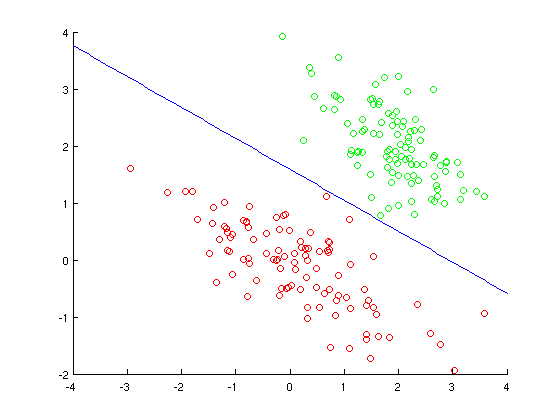
\includegraphics[scale = 0.4]{../Plottar/perceptron_example.png}
\caption{Example of a classification by Perceptron}
\label{fig:perceptron}
\end{figure}\\
%The basic idea for the Perceptron algorithm is for all input data, whose labeling are known, check their classification with the current weight vector. If the classification is correct, continue, else update the weight vector, $w$, according to Equation~\ref{eq:perceptron} \citep{perceptron_ai}.
%\begin{equation}
%\label{eq:perceptron}
%w = w + (x \cdot y)
%\end{equation}
%where $x$ is the input data and $y$ the desired output (1 or -1). The Perceptron algorithm converge when the weight vector remains unchanged \citep{perceptron_ai}. New data is classified by Equation~\ref{eq:new_perceptron}.
%\begin{equation}
%\label{eq:new_perceptron}
%class = sign(testData \cdot w)
%\end{equation}
%Where $class$ is the class the new data belongs to (1 or -1) and $w$ is the weight vector.\\\\
There is also another variant of the Perceptron algorithm, which is called Averaged Perceptron. They work in the same way, except that the Averaged Perceptron outputs the averaged weight vector instead of the final one.

\subsection{K-fold Cross Validation}
Cross Validation is used to test classification algorithms on sets of data that is unknown, in order to get an accurate evaluation of a hypothesis \citep{crossvalid_ai}.\\\\
K-fold cross validation means that the data is split into $k$ roughly equal sizes and then $k$ rounds of training is performed with $1/k$ as test data and the rest as training. The average score will be more accurate than one single score. K-values between 5 and 10 are popular and enough to get accurate results \citep{crossvalid_ai}.
